
\chapter{Results}
\label{sec:org8a9853f}

In this chapter the simulation results are presented with reference to the aim of the thesis, which was to study the mapping metrics:
their precision when assessing the mapping quality and their relation with the error amount after mapping.
First, in the \hyperref[sec:org13721de]{Impact of the mapping on the algorithm reliability} section we show how the mapping procedure affects the general increment of error.
After that, we analyze the metrics and their correlation with the error increase in the \hyperref[sec:orgc87040a]{Analysis of the mapping metrics} section.

\section{Impact of the mapping on the algorithm reliability}
\label{sec:org13721de}
After the selection of benchmarks in the \href{chapter-4.org}{Benchmarks} section, we started their simulations using our simulation framework.
Not surprisingly, some of the benchmarks either had very long simulation times or were even impossible to simulate in our lab servers. In most of those cases the circuits had more than ten qubits.
As we mentioned before throughout this thesis, the simulation of quantum systems is computationally exhausting.
The higher the number of qubits or the length of the circuit, the harder is it to simulate it.
Indeed, it is a critical issue in our case, as soon as we need to run multiple simulations in a complex error model.
Therefore, as can be seen in Tab. \ref{tab:map_selected_benchs}, we address that the final benchmark selection has a limitation in the number of qubits.

\begin{table}[htbp]
\caption{\label{tab:map_selected_benchs}
Table of the selected benchmarks to be mapped.}
\centering
\small
\begin{tabular}{lrrr}
\hline
Benchmark & \# qubits & \# gates & two-qubit gates (fraction)\\
\hline
\texttt{graycode6\_47} & 6 & 5 & 1.000\\
\texttt{xor5\_254} & 6 & 7 & 0.714\\
\texttt{4mod5\_v0\_20} & 5 & 20 & 0.500\\
\texttt{ham3\_102} & 3 & 20 & 0.550\\
\texttt{mod5d1\_63} & 5 & 22 & 0.591\\
\texttt{4gt11\_82} & 5 & 27 & 0.667\\
\texttt{rd32\_v0\_66} & 4 & 34 & 0.471\\
\texttt{alu\_v0\_27} & 5 & 36 & 0.472\\
\texttt{4mod5\_bdd\_287} & 7 & 70 & 0.443\\
\texttt{one\_two\_three\_v3\_101} & 5 & 70 & 0.457\\
\texttt{decod24\_bdd\_294} & 6 & 73 & 0.438\\
\texttt{alu\_bdd\_288} & 7 & 84 & 0.452\\
\texttt{one\_two\_three\_v1\_99} & 5 & 132 & 0.447\\
\texttt{mod10\_176} & 5 & 178 & 0.438\\
\texttt{4gt12\_v1\_89} & 6 & 228 & 0.439\\
\texttt{hwb4\_49} & 5 & 233 & 0.459\\
\texttt{4gt4\_v0\_72} & 6 & 258 & 0.438\\
\texttt{decod24\_enable\_126} & 6 & 338 & 0.441\\
\texttt{mod8\_10\_177} & 6 & 440 & 0.445\\
\texttt{mod5adder\_127} & 6 & 555 & 0.431\\
\texttt{sf\_276} & 6 & 778 & 0.432\\
\texttt{sf\_274} & 6 & 781 & 0.430\\
\texttt{sym6\_145} & 7 & 3888 & 0.438\\
\hline
\end{tabular}
\end{table}


As explained in the \href{chapter-4.org}{Analysis framework} section, after running the benchmarks for one thousand runs, the results obtained are the fidelity, the probability of success and the Quantum Volume.
We also extracted other metrics like the number of SWAPs added and the depth of the circuits, among other circuit statistics.
These metrics were obtained for all mentioned benchmarks before (non-mapped) and after mapping (mapped). 
Note that, for a fair comparison both the mapped and the non-mapped circuits were decomposed into the gates supported by  the Surface-17 chip (see Fig. \ref{fig:decompositions}). For the mapped ones, we used the three router algorithms developed in our group (see \hyperref[sec:org19dc500]{Mapping Model}): \textit{base}, \textit{minextend} and \textit{minextendrc}.

In quantumsim, we also tried different configurations regarding the decoherence time in order to study the mappers in different error regimes. 
All the results are shown in \href{appendix-1.org}{Appendix A}.


In order to illustrate how the mapping process affects the algorithm reliability, Figure \ref{fig:f_diff_bar_plot} shows the fidelity for some of the benchmarks before being mapped and after being mapped using the \texttt{minextendrc} router.
We can see how the fidelity is smaller for long circuits -- like \texttt{sf\_274} or \texttt{mod5adder\_127} -- than for the short ones -- \texttt{graycode6\_47} or \texttt{xor5\_254}.
It can be seen how, for the long circuits, the fidelity decreases more than 50\%.
For instance, \texttt{sf\_274}'s fidelity goes from 0.35 to 0.17 or \texttt{mod5adder\_127}'s goes from 0.45 to 0.19.
On the other hand, for the small circuits like \texttt{graycode6\_47} or \texttt{xor5\_254} the fidelity decreases around 1\%; from 0.99 to 0.98 and from 0.99 to 0.97, respectively.
For more details, we show the exact result values for all the benchmarks in \href{appendix-1.org}{Appendix A}.

\begin{figure}[htbp]
\centering
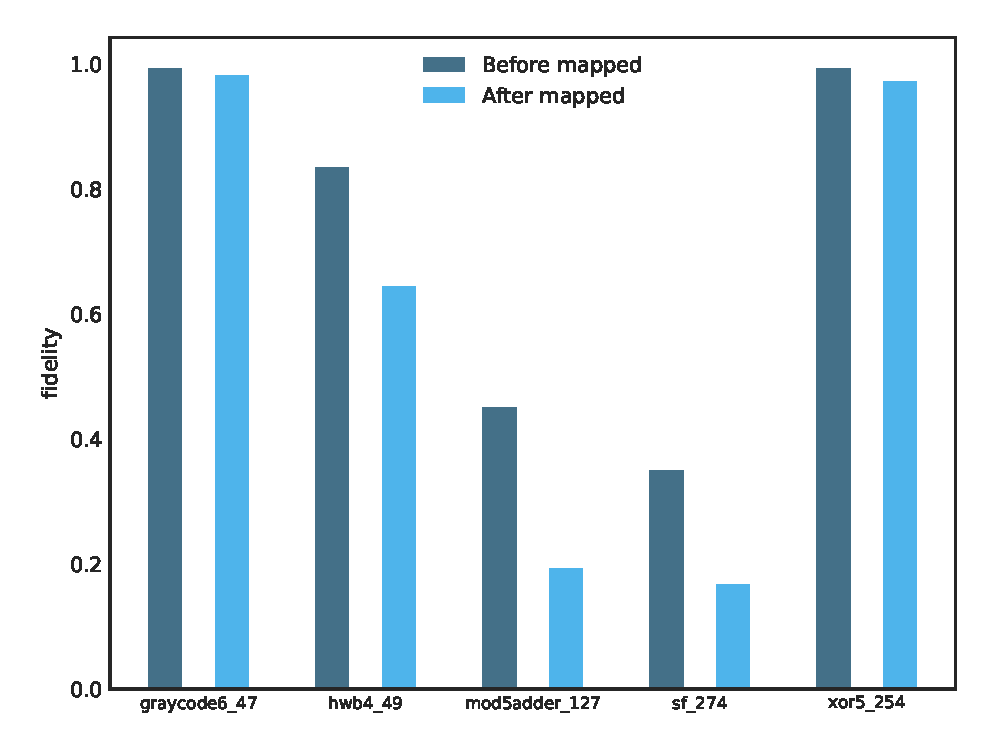
\includegraphics[width=0.7\textwidth]{figures/f_diff_bar_plot.eps}
\caption{\label{fig:f_diff_bar_plot}
Difference of fidelities before and after mapping with the \emph{minextendrc} router for five different benchmarks.}
\end{figure}
As we mentioned before, we use three different routers, each one giving a different mapped version per benchmark and, therefore, different metric statistics.
For instance, as it can be seen in \href{appendix-1.org}{Appendix A} and in Tab. \ref{tab:depth_per_bench}, the depth of the \texttt{graycode6\_47} circuit before being mapped is 32 cycles and after being mapped grows to 111, 61 or 82 depending on the router.
In Fig. \ref{fig:mapping_effect_3000_diff_lines} and Fig. \ref{fig:mapping_effect_1000_diff_lines} we plot the fidelity of each benchmark, where the dots are the different benchmark configurations aligned vertically and ordered from the shortest to the longest circuit depth; from left to right.
The dark blue dots represent the benchmarks before being mapped and the light blue ones represent the different mapped version of it from the different routers.
Each figure represents simulations with a different decoherence time, Fig. \ref{fig:mapping_effect_3000_diff_lines} presents the result with a decoherence time of \(30 \mu s\) and Fig. \ref{fig:mapping_effect_1000_diff_lines} the ones with a decoherence time of \(10 \mu s\).
As mentioned in the \href{quantum_computing.org}{Qubits are faulty} section, the shorter the decoherence time the more errors would appear and the faster a qubit will be not useful.

In Fig. \ref{fig:mapping_effect_diff_3000} and Fig. \ref{fig:mapping_effect_diff_1000} we plot the maximum (red) and minimum (blue) percentage of difference in fidelity between the non-mapped version of the benchmarks and each one of the mapped versions.
We calculate the percentage of the fidelity difference as the ratio between the difference in fidelities and the fidelity of the non-mapped version \(\left(\frac{f_{\text{before}} - f_{\text{after}}}{f_{\text{before}}}\right)\).
As an example, in Fig. \ref{fig:mapping_effect_3000_diff_lines} and Fig. \ref{fig:mapping_effect_1000_diff_lines}, we plot two lines over some benchmark to depict the maximum (red) and the minimum(blue) difference per benchmark.

Finally, in Tab. \ref{tab:depth_per_bench} we show the exact depth values of each one of the benchmarks in the order they appear, from left to right.
For instance, the first column of dots to the left is the \texttt{graycode6\_47} circuit.



From these results, we observe that, in general, the fidelity starts from lower points just as the size of the circuit increases.
This behaviour is certainly because the longer the circuit, the more errors it will get.
We can also observe how the fidelity difference between non-mapped and the mapped algorithms tends to grow.
Due to most of the selected benchmarks have a similar two-qubit gates percentage and also a similar number of qubits -- main parameters for the mapping task --, we can say that this increasing tendency is mostly provoked by the length of the circuit at the very beginning.
Or what is the same, that if a circuit is already long before mapping, the results of the mapped version will be bad, no matter which mapper is used.
For instance, let us assume two different circuits with a similar number of qubits and the same percentage of two-qubit gates, but different circuit depths, one much longer than the other.
While mapping them, the router will have the same proportion of two-qubit interactions and, therefore, the mapper will act similarly in both cases.
But, based on our results, the difference in fidelity between the mapped and non-mapped versions of the short algorithm will be much smaller than the difference in fidelity between the mapped and non-mapped versions of the long circuit.
Moreover, another remark we see is that, in the case of a decoherence time of \(10 \mu s\) (Fig \ref{fig:mapping_effect_1000}), we observe strange results like negative fidelities. 
This is due to the chaotic behaviour of the quantum noise; the more it affects the system, the more chaotic results appear.


\begin{figure}
\centering
\subfigure[Fidelity per benchmark]{

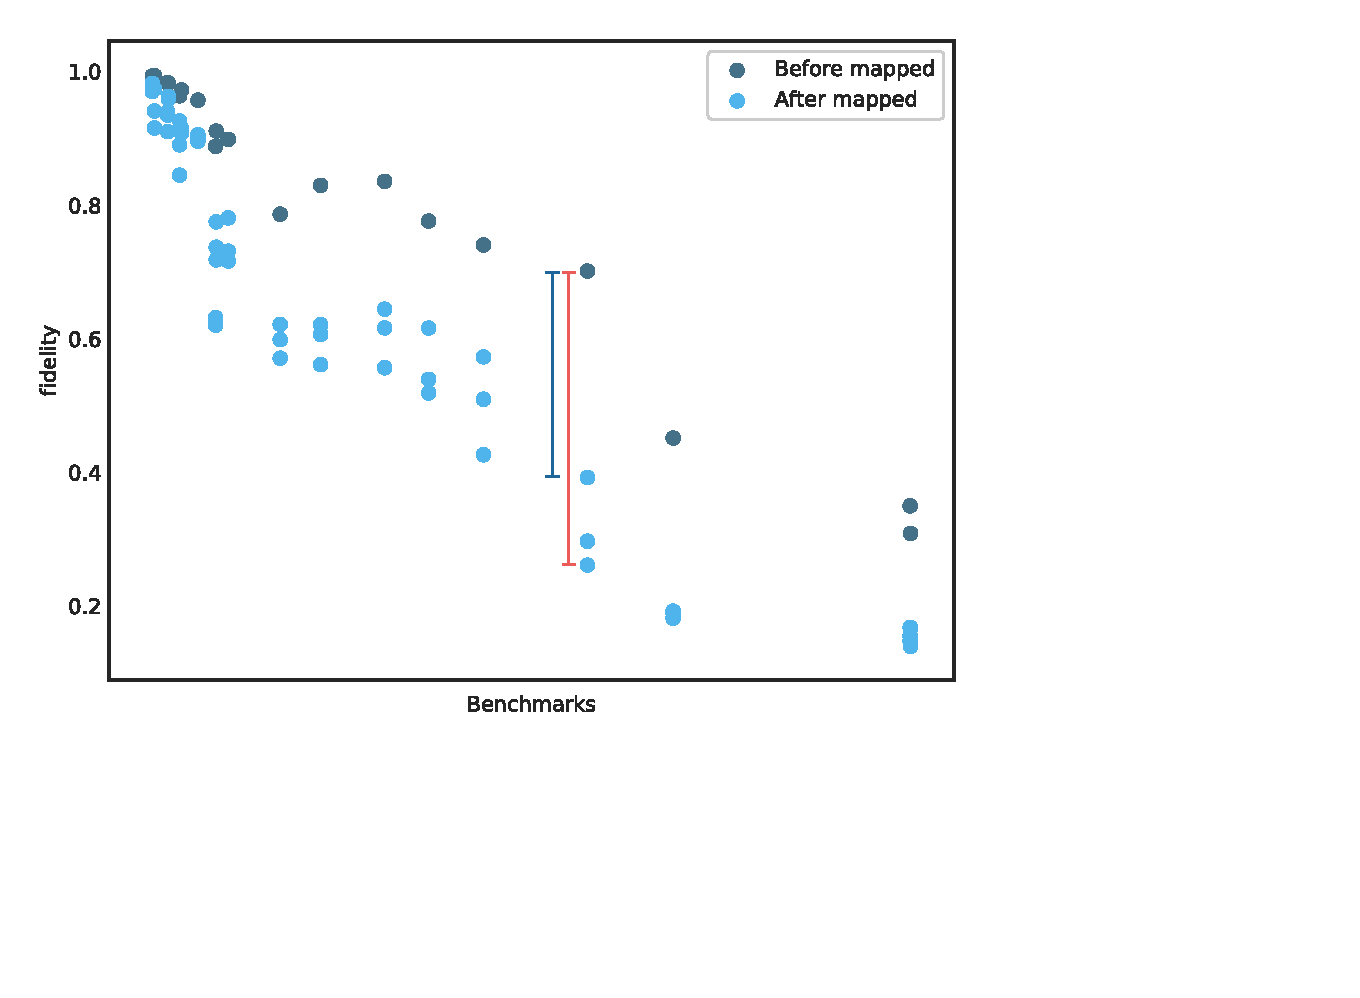
\includegraphics[width=0.7\textwidth]{figures/mapping_effect_3000_diff_lines.eps}

\label{fig:mapping_effect_3000_diff_lines}
}

\subfigure[Difference of fidelity per benchmark]{

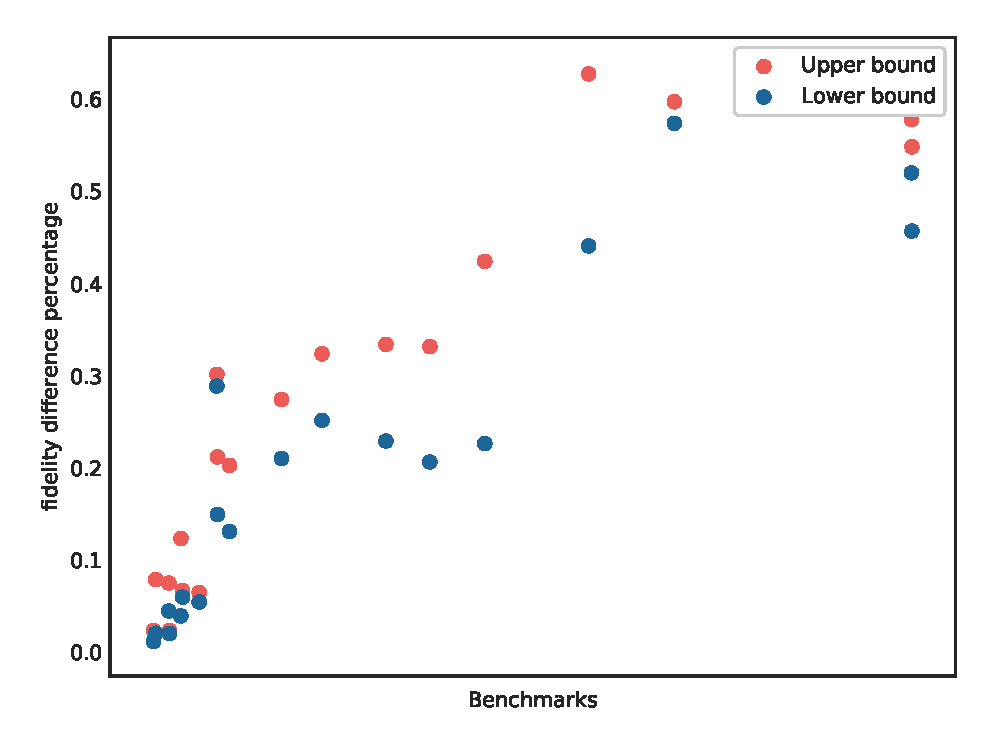
\includegraphics[width=0.7\textwidth]{figures/mapping_effect_diff_3000.eps}

\label{fig:mapping_effect_diff_3000}
}

\caption{Impact of mapping for $t_d = 30 \mu s$}
\label{fig:mapping_effect_3000}
\end{figure}


\begin{figure}
\centering
\subfigure[Fidelity per benchmark]{

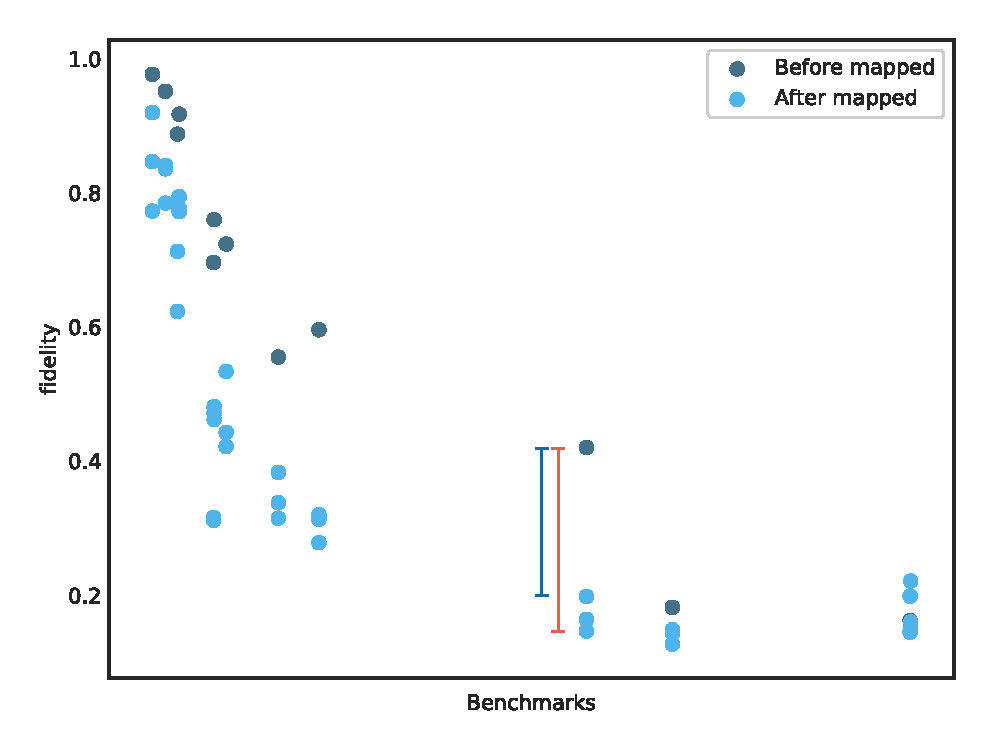
\includegraphics[width=0.7\textwidth]{figures/mapping_effect_1000_diff_lines.eps}

\label{fig:mapping_effect_1000_diff_lines}
}

\subfigure[Difference of fidelity per benchmark]{

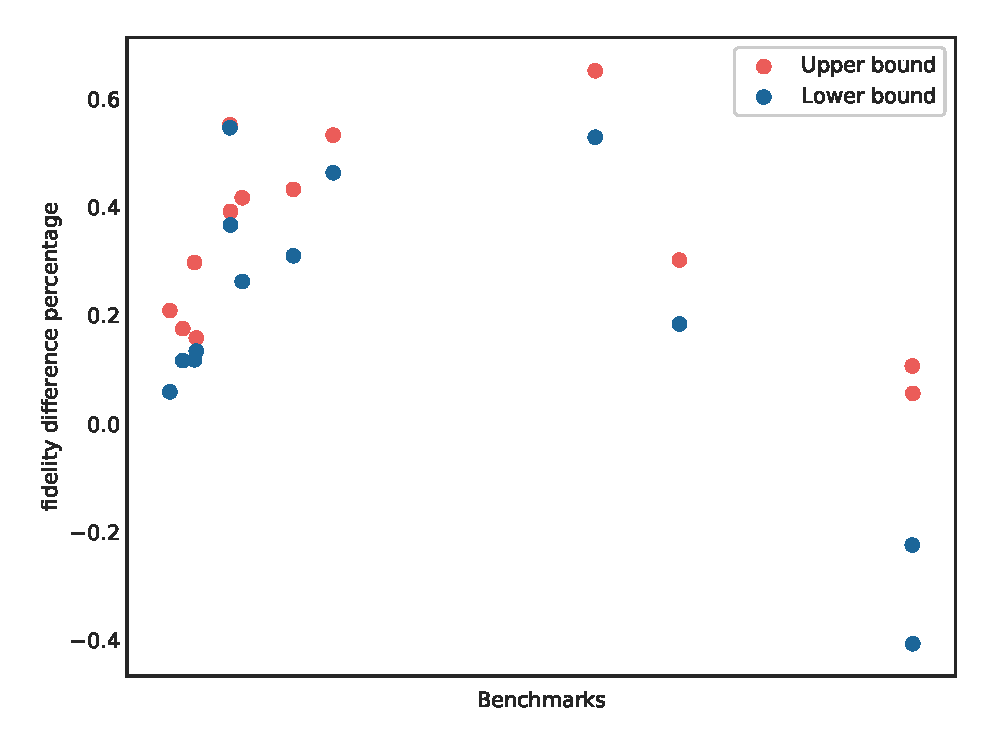
\includegraphics[width=0.7\textwidth]{figures/mapping_effect_diff_1000.eps}

\label{fig:mapping_effect_diff_1000}
}

\caption{Impact of mapping for $t_d = 10 \mu s$}
\label{fig:mapping_effect_1000}
\end{figure}


\begin{table}[htbp]
\caption{\label{tab:depth_per_bench}
Different depth per benchmark}
\centering
\tiny
\begin{tabular}{lrrrr}
\hline
Benchmark & Depth before mapping & Depth after mapping with \emph{minextendrc} & Depth after mapping with \emph{minextend} & Depth after mapping with \emph{base}\\
\hline
\texttt{graycode6\_47} & 32 & 111 & 61 & 82\\
\texttt{mod5d1\_63} & 59 & 209 & 136 & 146\\
\texttt{ham3\_102} & 60 & 127 & 121 & 98\\
\texttt{alu\_v0\_27} & 80 & 248 & 156 & 214\\
\texttt{miller\_11} & 112 & 307 & 278 & 231\\
\texttt{one\_two\_three\_v3\_101} & 143 & 440 & 302 & 323\\
\texttt{decod24\_bdd\_294} & 144 & 407 & 328 & 300\\
\texttt{alu\_bdd\_288} & 165 & 495 & 383 & 360\\
\texttt{one\_two\_three\_v1\_99} & 256 & 839 & 530 & 609\\
\texttt{mod10\_176} & 327 & 1090 & 687 & 734\\
\texttt{hwb4\_49} & 439 & 1387 & 961 & 1006\\
\texttt{mini\_alu\_167} & 516 & 1598 & 992 & 1274\\
\texttt{decod24\_enable\_126} & 612 & 1788 & 1440 & 1446\\
\texttt{mod8\_10\_177} & 794 & 2275 & 1761 & 2006\\
\texttt{mod5adder\_127} & 944 & 2878 & 2667 & 2378\\
\hline
\end{tabular}
\end{table}

\section{Analysis of the mapping metrics}
\label{sec:orgc87040a}
Once we acknowledge the behaviour of the error growth due to the mapping process, it is time to understand which circuit parameter affects it the most.
In this section we evaluate the behaviour and quality of the mapping metrics.
From the common ones -- number of SWAPs and depth -- to the ones we proposed -- fidelity, probability of success and Quantum Volume.



First we analyze the probability of success and fidelity correlation.
As we explained in the \hyperref[sec:org0c7b2c2]{Fidelity and Probability of success}, the main difference between them is that the probability of success takes into account the errors related with the measurement of the qubits but, unlike fidelity, is not able to calculate errors in quantum states.

As expected, our experiments prove that both metrics are highly correlated.
We also appreciated the fact that the probability of success, in general, is higher than the fidelity.
This could suggest that the measurement is 'correcting' circuit errors colliding the state in the correct result, instead of the wrong one.
It is a 'good' mistake that results in the expected solution.
Nevertheless, this behaviour could be caused by the fact that our algorithms are deterministic.
Another observation is that the closer the values are to 0 the more chaotic and random the values get.



[TWO PARTS IN THE GRAPH  LINEARITY AND RANDOM: \textcolor{red}{this is contrary to being logarithmic}]

[EXPLAIN INHERENT BEHAVIOUR OF THE MEASUREMENT FOR THE CHAOTIC PART OF THE GRAPH]

In Fig. \ref{fig:f_ps_correlation_with_meas_error} we plot the results of the framework in terms of probability of success and fidelity. 
For this figure and the figures from now on in this section, each dot is a different benchmark configuration (see \href{appendix-1.org}{Appendix A}) and the colors represent different decoherence times, blue for 30 \(\mu s\) and orange for 10 \(\mu s\).
As we explained in the \href{quantum_computing.org}{Qubits are faulty} section, the shorter the decoherence time the more errors will appear in our quantum system.
Fig. \ref{fig:f_ps_correlation_with_meas_error} highlights a correlation with a bias between both metrics, proving the fact that the probability of success is always higher than the fidelity.
For instance, for values around 0.6 in fidelity, the probability of success has a value bigger than 0.7 for the majority of the samples.
This behaviour could be due to the small error rate the measurement has.
Note that for values close to 1, fidelity and probability of success tend to be almost equal and linear, which make sense; if some circuit has almost no error, both metrics will be equally good.
At the same time, the closer the values are to 0, the more spread the samples are, proving the chaotic and random behaviour.
It can be seen that the curvature of the fitting line changes depending on the decoherence time of the system.
For higher error rates -- orange function --, the curve tends to decrease faster; what means that the higher the error rates the less fidelity and probability of success the circuits will get.
The cluster that appears between the 0.9 and 1.0 values is due to the amount of simple benchmarks in the selection, as we previously mentioned.

\begin{figure}[htbp]
\centering
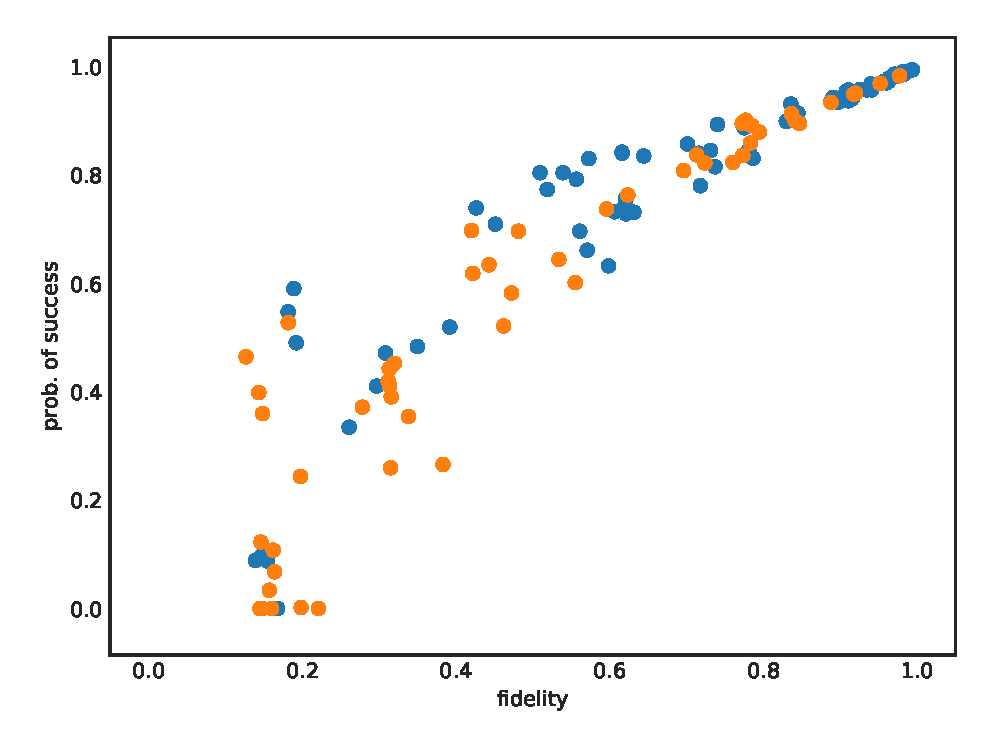
\includegraphics[width=0.7\textwidth]{figures/f_ps_correlation.eps}
\caption{\label{fig:f_ps_correlation_with_meas_error}
Correlation between fidelity and probability of success for two different decoherence times}
\end{figure}



Regarding the rest of the metrics, we analyzed their relation with the fidelity and probability of success.
Instead of using the number of SWAPs we decided to use the number of two-qubit gates because we noticed in the results that the number of gates \textcolor{red}{Do you mean number of any gates or just number of two-qubit gates? Because the latter}in the circuit before being mapped is important in this analysis.
For instance, it is not the same to add 10 SWAPs to a circuit with 100 operations than one with 10000.


The results of the main mapping metrics against fidelity are depicted in Fig. \ref{fig:f_metrics_correlation}.
We observe that, for all the cases, the fidelity decreases with an inverse exponential behaviour and that it decreases faster for small decoherence times.
Certainly, the shorter the decoherence times we use the more benchmarks will have non-useful results.
We can also see how fidelity never goes to zero, but it gets constant around 0.2, giving random results.
We consider the point where fidelity is constant as the limit in terms of each one of the variables.
We plot a line for the orange samples to mark this point.
Finally, it can be seen how the number of gates is the metric most related with the fidelity; it is the one with the samples more ordered.

\begin{figure}[htbp]
\centering
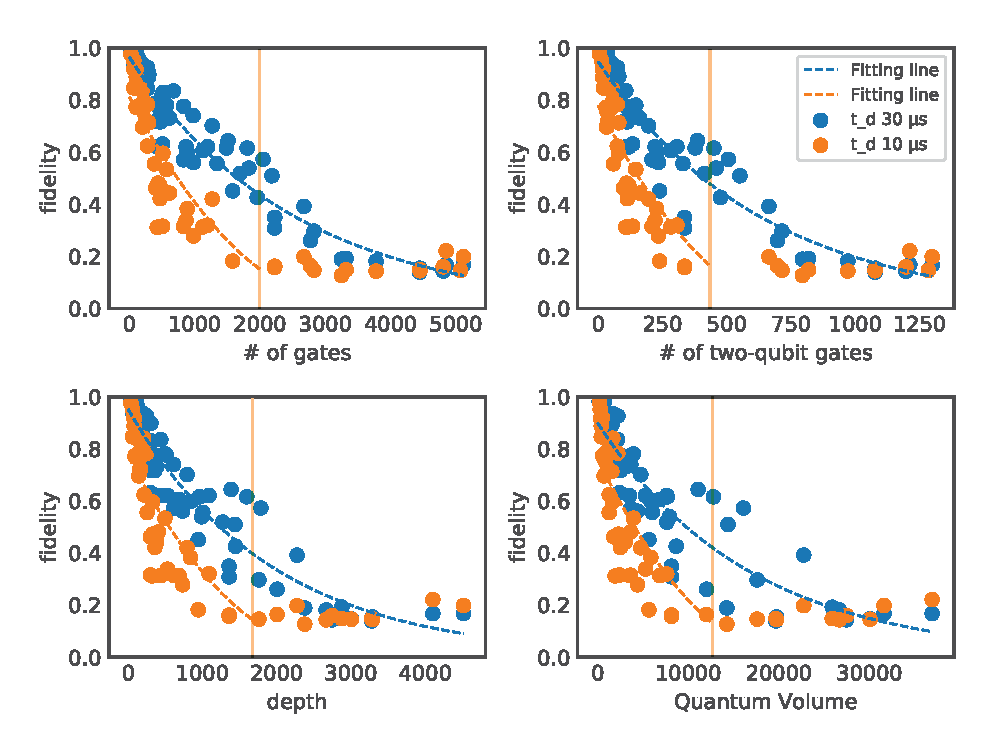
\includegraphics[width=\textwidth]{figures/f_metrics_correlation_poly.eps}
\caption{\label{fig:f_metrics_correlation}
Correlation between fidelity and the mapping metrics.}
\end{figure}

The correlation between the probability of success and the other metrics can be see in Fig. \ref{fig:ps_metrics_correlation}.
We also observe a decreasing behaviour, although the shape is not as clear as in the case of fidelity.
This could be provoked, again, by the final error added by the measurement gate and by the fact that, most of the times, the measurement is correcting the wrong solutions.
The figure also highlights how the fast probability of success decreases depending on the decoherence time.

\begin{figure}[htbp]
\centering
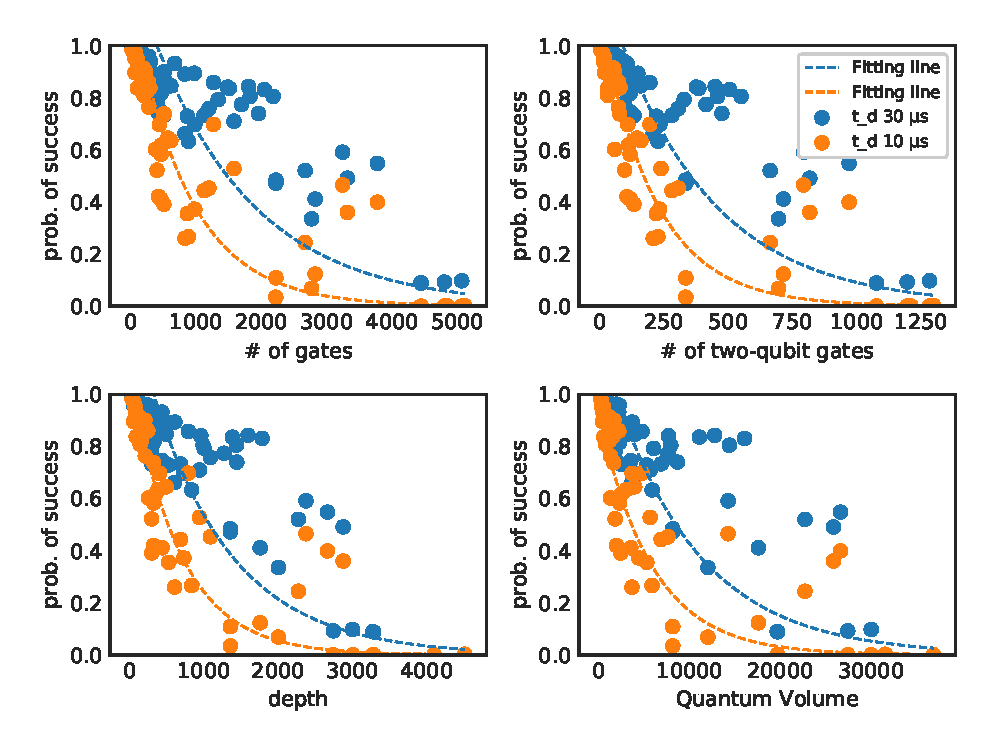
\includegraphics[width=\textwidth]{figures/ps_metrics_correlation.eps}
\caption{\label{fig:ps_metrics_correlation}
Correlation between probability of success and the mapping metrics.}
\end{figure}

We can also see in both figures that, as announced before, there is a cluster of benchmarks with high fidelity and high probability of success.
This happens because of the high concentration of small benchmarks, due to the simulation difficulties.
On the contrary, the rest of the values are a bit spread.
In general, we observe a high correlation between all of the metrics; so in order to get correlation quality values to differ between the metrics, we calculated the Pearson correlation coefficient.
Note that the Pearson coefficient measures linear correlations and, as it will be seen in Fig. \ref{fig:f_metrics_correlation}, the metrics behave in an inverse exponential fashion against fidelity.
For this reason, we applied a \(log\) transformation to our fidelity data in order to make it linear for the Pearson calculation.


As it can be seen in the Pearson values (Tab. \ref{tab:pearson_corr_f} and Tab. \ref{tab:pearson_corr_ps}) the most correlated metric is the number of two-qubit gates.
These results hold the fact that the quality of the mapping depends directly on the length of the targeted circuit before it is being mapped.
For example, a long circuit well mapped will have always worse results in fidelity or probability of success than a short circuit badly mapped.
As Tab. \ref{tab:pearson_corr_f} and Tab. \ref{tab:pearson_corr_ps} highlight, we have a worse correlation for the shorter decoherence time.
This lack of correlation can be attributed to the fact that the majority of the samples with \(t_d = 1000\) are highly affected by the errors and, therefore, the samples have more random values.
Moreover, contrary to expectations, the Quantum Volume was the least correlated metric.
This small lack of correlation can be attributed to the imprecise formula that we chose to calculate it.
Future work needs to be done to inspect a better formula.
Finally, if we compare both tables, we can see that the fidelity is more correlated with the metrics that the probability of success.
It is very likely that the reason for this result is that the added measurement error distribution in the end of the circuit adds more noise and spreads our samples.
Also the 'correcting' errors behaviour of the measurement should be taken into account.

\begin{center}
\captionof{table}{\label{tab:pearson_corr_f}
Pearson correlation coefficient of the log transformation of fidelity against the metrics(\(\rho _{log(f),Y}\)), where \(Y\) is one of the four metrics we analyze}
\begin{tabular}{lrrrr}
\hline
 & \# of Gates & \# of Two-qubit gates & Depth & \(V_Q\)\\
\hline
\(t_d = 3000\) & -0.9730 & -0.9600 & -0.9455 & -0.9118\\
\(t_d = 1000\) & -0.8466 & -0.8135 & -0.8093 & -0.7736\\
\hline
\end{tabular}
\end{center}

\begin{center}
\captionof{table}{\label{tab:pearson_corr_ps}
Pearson correlation coefficient for the probability of success against the metrics (\(\rho _{p_s,Y}\)), where \(Y\) is one of the four metrics we analyze}
\begin{tabular}{lrrrr}
\hline
 & \# of Gates & \# of Two-qubit gates & Depth & \(V_Q\)\\
\hline
\(t_d = 3000\) & -0.9363 & -0.9248 & -0.9179 & -0.8797\\
\(t_d = 1000\) & -0.8341 & -0.8097 & -0.8076 & -0.7686\\
\hline
\end{tabular}
\end{center}
